\documentclass[11pt]{article}
\ifdefined\pdfsuppresswarningpagegroup
\pdfsuppresswarningpagegroup=1
\fi

\usepackage[a4paper,margin=1in]{geometry}
\usepackage{amsmath,amssymb}
\usepackage{graphicx}
\usepackage{booktabs}
\usepackage{array}
\usepackage{float}
\usepackage[hidelinks]{hyperref}
\usepackage{xcolor}
\usepackage{microtype}
\usepackage{caption}

\title{Construction Sensitivity of Shortest-Path Anisotropy Diagnostics\\
in Geometric Graphs from Black-Hole Embeddings}
\author{Ariadna Uxue Palomino Ylla\\
Department of Physics, Nagoya University, Nagoya, Japan\\
\texttt{palomino.ylla.ariadna.uxue.e8@s.mail.nagoya-u.ac.jp}}
\date{}

\newcommand{\clog}{C_{\log}}
\newcommand{\drho}{\Delta\rho_r}

\begin{document}

\maketitle

\begin{abstract}
Geometric graphs provide flexible discretizations of sampled spaces, but graph
observables can depend strongly on the sampling rule, edge construction, and
choice of control. This makes it difficult to determine whether an apparent
geometric signal is a property of the sampled space or of the graph-building
protocol. We study this problem using graph discretizations of embedded spatial
slices of static black-hole geometries as controlled benchmarks.

We focus on a shell-based shortest-path anisotropy statistic, $\clog$, defined
as the cubic mean deviation of logarithmic shortest-path multiplicities over
finite graph-distance shells. Ten-seed Bardeen and Hayward parameter scans show
organized but realization-dependent radial behavior under the original
calibrated construction. We perform paired five-protocol audits at
Schwarzschild/Flamm, Bardeen $g=0.2$, and Hayward $\ell=0.2$ using
five graph/control protocols: the original matched-flat KNN convention, strict
radius-threshold controls, pure KNN graphs, mutual KNN graphs, and
edge-count-matched radius graphs. In every run the black-hole graph and its
controls reuse the same radial-angular sample, and correlations are computed
from twelve common radial bins.

For Schwarzschild, the mean absolute black-hole/control correlation gaps are
$0.242\pm0.161$, $0.688\pm0.442$, $0.233\pm0.199$,
$0.422\pm0.323$, and $0.681\pm0.445$ for the original, strict-radius,
pure-KNN, mutual-KNN, and edge-matched-radius protocols, respectively
(mean $\pm$ standard deviation over ten seeds). Radius-style controls therefore
do not erase the separation; they give the largest average magnitudes in the
audited sample. The Bardeen and Hayward anchors reproduce this qualitative
construction dependence: their original mean absolute gaps are $0.255\pm0.174$
and $0.250\pm0.165$, whereas edge-matched-radius gaps are $0.676\pm0.452$ and
$0.680\pm0.443$. Signed gaps vary across realizations and protocols.

Thus, the black-hole/control separation is neither graph-construction invariant
nor realization independent. $\clog$ is a reproducible finite-graph statistic
when the sampling, edge rule, shell radius, binning, seed, and null model are
specified, but the present evidence does not support interpreting it as a
graph-independent curvature scalar. More broadly, the results motivate a
matched-control audit framework in which geometric claims are attached to a
complete diagnostic--construction--control protocol.
\end{abstract}

\section{Introduction}

Geometric graphs are widely used as finite representations of sampled metric
spaces, spatial data, and physical or data-driven geometries
\cite{Penrose2003,DallChristensen2002,Newman2010}. However, a graph observable
measured on such a representation is rarely a function of geometry alone. It can
also depend on sampling density, boundary effects, edge rule, graph scale, and
null model. Similar difficulties appear in thresholded and density-controlled
network analyses, where changing the graph construction can change the
interpretation of a measured network statistic
\cite{VanWijk2010,Langer2013,Ginestet2011}. For this reason, geometric
interpretations of graph diagnostics require matched controls and explicit
construction-sensitivity tests.

This issue is related, but not identical, to the problem of defining curvature
on discrete structures. Classical discretizations such as Regge calculus encode
curvature through a specific discretized geometric framework \cite{Regge1961}.
Graph and cell-complex notions such as Forman and Ollivier Ricci curvature
provide alternative discrete analogues with different mathematical meanings
\cite{Forman2003,Ollivier2009}. The present work takes a complementary
approach. We do not attempt to define a new discrete curvature tensor or scalar.
Instead, we ask when a shortest-path graph diagnostic displays geometric
organization and whether that organization survives stricter matched-control
tests.

We use embedded spatial slices of black-hole geometries as a controlled setting
for this question. These surfaces provide smooth radial benchmarks rather than
new astrophysical predictions. The benchmark families are the
Schwarzschild/Flamm embedding and two regular black-hole models, Bardeen and
Hayward \cite{Schwarzschild1916,Flamm1916,Bardeen1968,Hayward2006}. Under the
original fixed construction, representative graphs from all three families show
closely aligned radial $\clog$ profiles. This observation motivates, but does
not by itself establish, a construction-independent geometric signal.

The diagnostic $\clog$ measures the dispersion of logarithmic shortest-path
multiplicities over a finite graph-distance shell. An earlier
single-realization construction sweep suggested that the black-hole/control gap
was large under the original matched-flat KNN control and almost vanished under
radius-style controls. The purpose of the present revision is to test that
interpretation with a paired multi-seed audit and a single canonical correlation
pipeline. The audit shows that the earlier collapse was not representative:
strict-radius and edge-matched-radius controls instead produce the largest mean
absolute gaps, while realization-to-realization variability is substantial.

The scientific message is therefore not that one construction is uniquely
correct. The separation depends jointly on the diagnostic, graph construction,
and control. We distinguish three logically different questions:
(i) reproducibility within a fixed protocol, (ii) sensitivity across protocols,
and (iii) invariance under graph construction. The ten-seed experiment quantifies
the first two and does not support the third.

We report canonical ten-seed fixed-protocol scans for Bardeen and Hayward and
representative five-protocol audits for both families. These data separate
reproducibility within a protocol from sensitivity across constructions; they
do not establish graph-independent curvature invariance.

\section{Graph benchmarks and matched controls}

\subsection{Embedding geometries}

We consider geometric graphs sampled from embedded spatial slices of static
black-hole benchmark geometries. For a static, spherically symmetric metric
written as
\begin{equation}
    ds^2 = -f(r)dt^2 + f(r)^{-1}dr^2 + r^2d\Omega^2,
\end{equation}
the equatorial spatial slice has line element
\begin{equation}
    dl^2 = f(r)^{-1}dr^2 + r^2d\phi^2 .
\end{equation}
Embedding this slice as a surface of revolution in Euclidean three-space gives
\begin{equation}
    dl^2 =
    \left(1+\left(\frac{dz}{dr}\right)^2\right)dr^2+r^2d\phi^2,
\end{equation}
and therefore
\begin{equation}
    \frac{dz}{dr} =
    \sqrt{\frac{1}{f(r)}-1}.
\end{equation}

The Schwarzschild case uses
\begin{equation}
    f_{\mathrm{Schw}}(r) = 1-\frac{2M}{r}.
\end{equation}
For the Bardeen regular black-hole family, we use
\begin{equation}
    f_{\mathrm{B}}(r)
    =
    1-\frac{2Mr^2}{(r^2+g^2)^{3/2}},
\end{equation}
and for the Hayward family,
\begin{equation}
    f_{\mathrm{H}}(r)
    =
    1-\frac{2Mr^2}{r^3+2M\ell^2}.
\end{equation}
The scans use $M=1/2$, $g\in\{0,0.1,0.2,0.3\}$, and
$\ell\in\{0,0.1,0.2,0.3\}$. The five-protocol anchors use $g=0.2$ and
$\ell=0.2$.

\subsection{Matched-flat controls}

For each black-hole graph, matched-flat controls reuse the same radial and
angular samples. The flat control removes the embedded height,
\begin{equation}
    (r,\phi,z(r)) \longrightarrow (r,\phi,0),
\end{equation}
while preserving the radial-angular sampling. The control therefore asks how
much of the diagnostic organization remains after replacing the curved
embedding by a flat geometry with the same sampling information.

The graph-construction rule is part of the protocol. A diagnostic value is not
interpreted independently of the edge rule and null model; every comparison is
treated as a diagnostic--construction--control triple.

\begin{figure}[H]
    \centering
    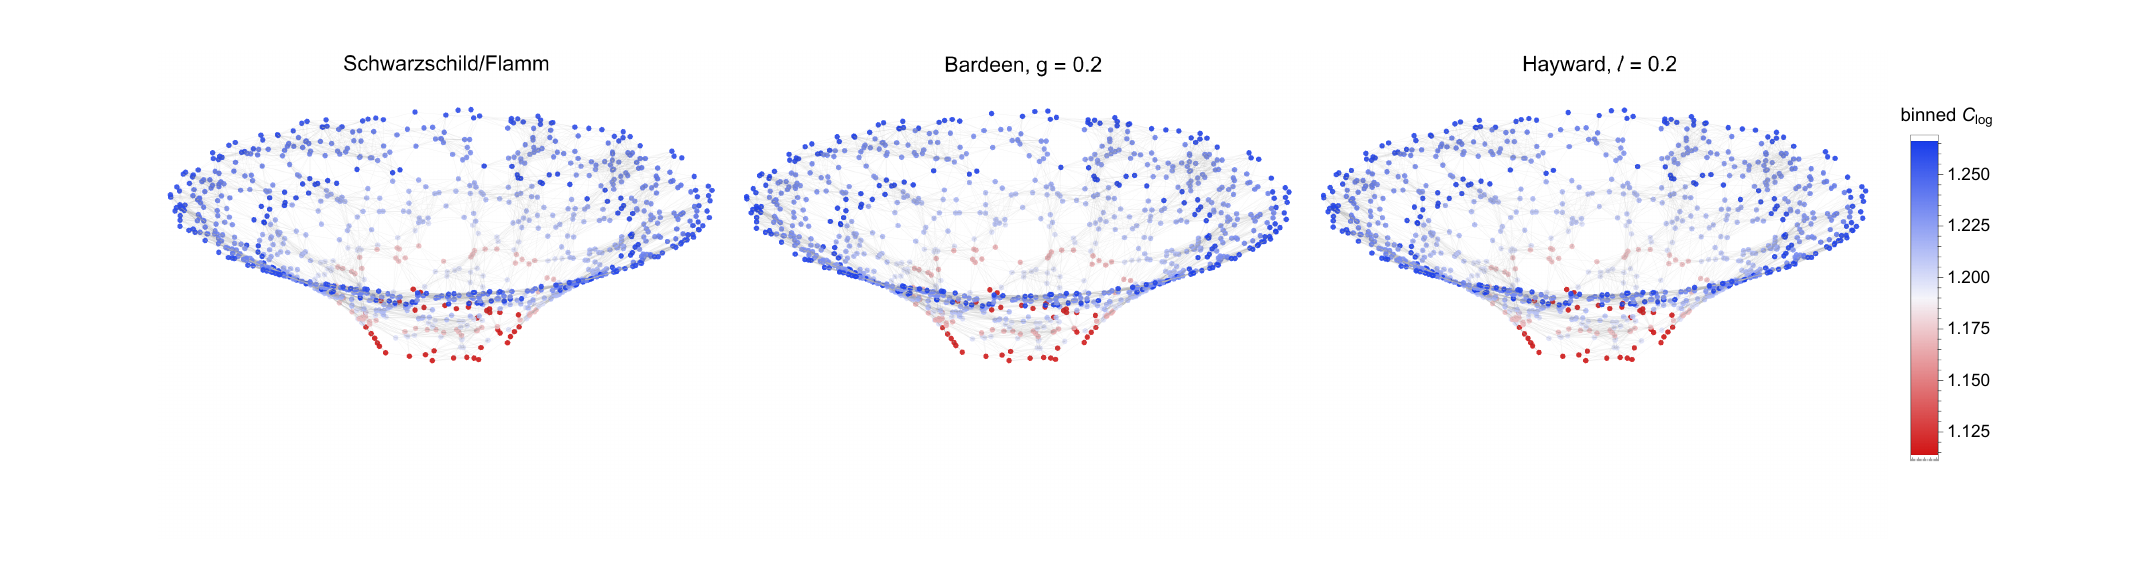
\includegraphics[width=0.98\linewidth]{results/figures/black_hole_family_colored_by_LogCMD_3models_smoothed.png}
    \caption{Representative Schwarzschild/Flamm, Bardeen ($g=0.2$), and Hayward
    ($\ell=0.2$) embedding graphs, colored by radially binned mean $\clog$ on a
    common scale. These fixed-protocol visualizations motivate the broader
    family program; they are not a substitute for the paired multi-protocol
    audit reported below.}
    \label{fig:bh-family-graph-visualization}
\end{figure}

\begin{figure}[H]
    \centering
    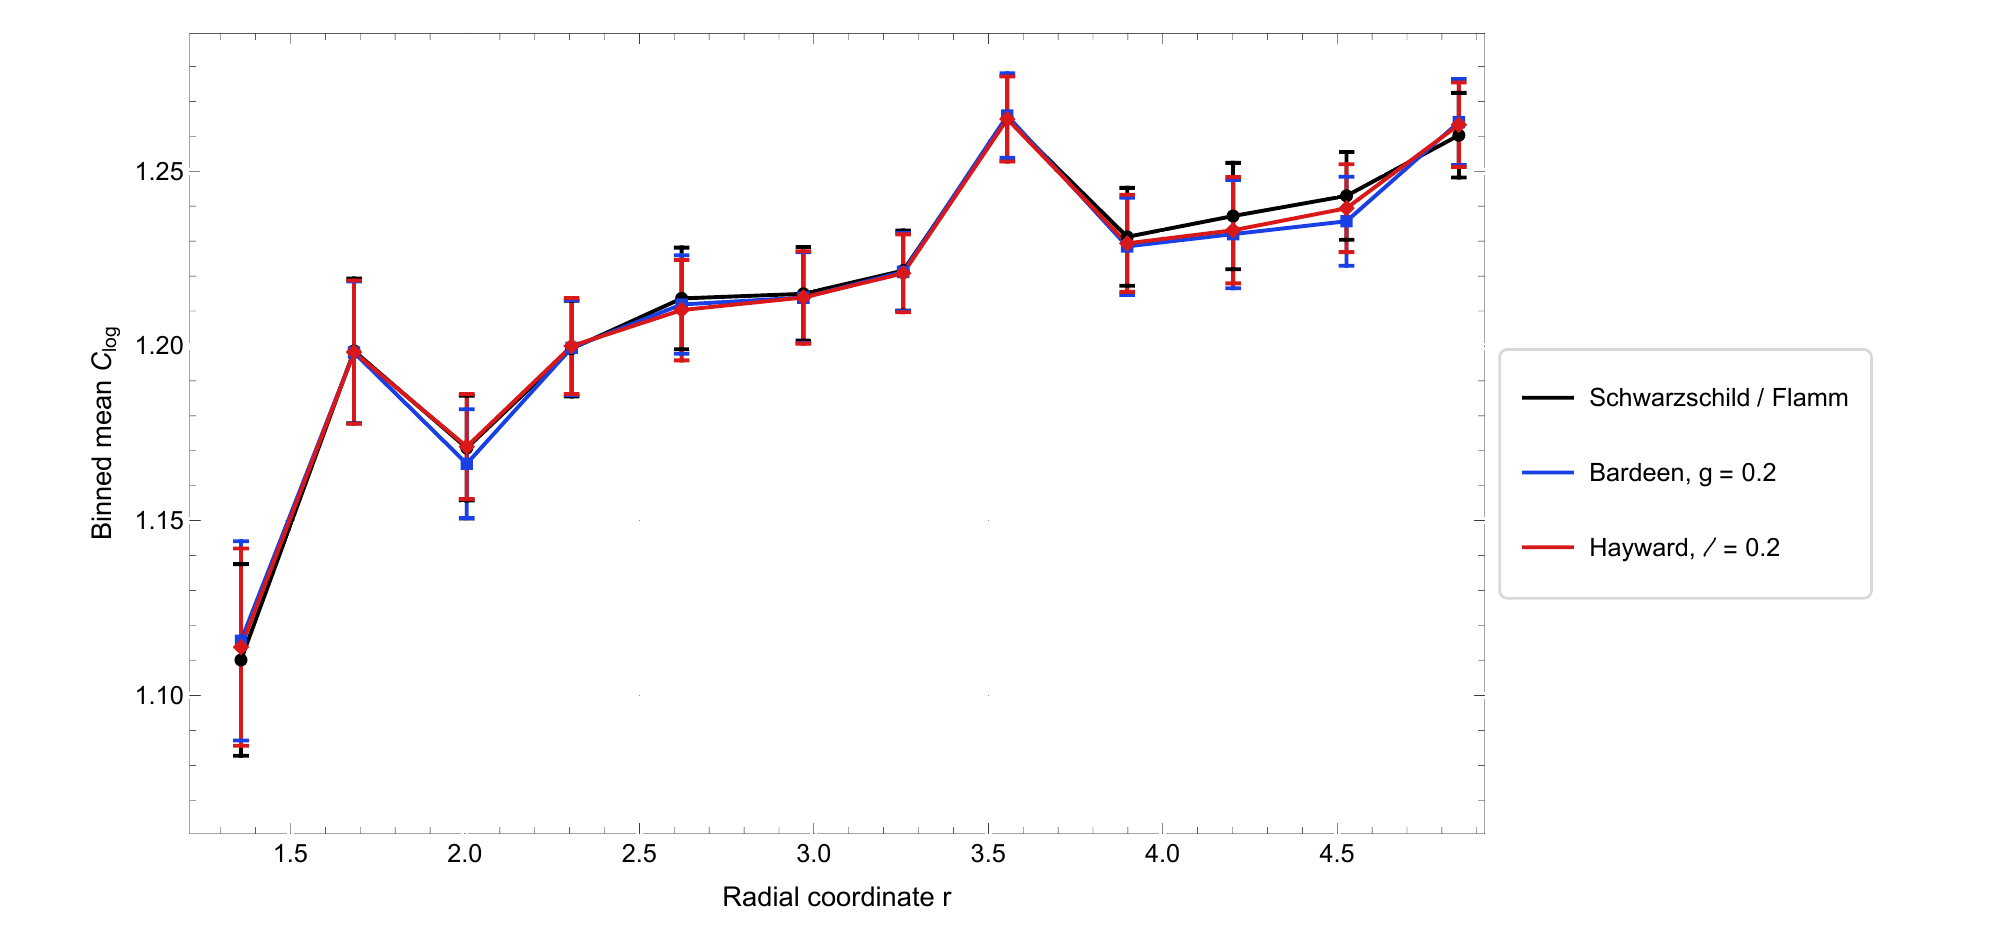
\includegraphics[width=0.94\linewidth]{results/figures/black_hole_family_radial_profile_plot3.png}
    \caption{Representative binned radial $\clog$ profiles for the three
    benchmark families under the original calibrated construction. The close
    alignment shows that the motivating radial organization is not visually
    unique to Schwarzschild; the canonical scans and anchor audits below provide
    the quantitative family comparison.}
    \label{fig:bh-family-radial-profiles}
\end{figure}

\section{Shortest-path anisotropy diagnostic}

Let $G=(V,E)$ be a finite graph and let $d_G(i,j)$ denote graph distance. For a
reference vertex $i$ and graph-shell radius $r_g$, define
\begin{equation}
    S_{r_g}(i) = \{j \in V : d_G(i,j)=r_g\}.
\end{equation}
Let $m_{ij}$ be the number of shortest paths between $i$ and $j$. The statistic
$\clog$ is the cubic mean deviation of the logarithmic multiplicities over the
shell,
\begin{equation}
    \clog(i;r_g)
    =
    \left(
    \frac{1}{|S_{r_g}(i)|}
    \sum_{j\in S_{r_g}(i)}
    \left|
    \log m_{ij} - \langle \log m \rangle_{S_{r_g}(i)}
    \right|^3
    \right)^{1/3}.
    \label{eq:clog}
\end{equation}
This quantity probes anisotropy in shortest-path multiplicity patterns rather
than degree or edge density alone. It is a finite-shell graph observable, not a
continuum scalar by definition.

\subsection{Canonical numerical protocol}
\label{sec:numerical-protocol}

All audited graphs use $M=1/2$, $N=1000$, construction parameter $k=16$,
graph-shell radius $r_g=3$, twelve common radial bins, and seeds 1--10. One
radial-angular sample is generated per family, parameter, and seed. Its flat
control reuses that sample; at each anchor the same sample is also reused by all
five graph/control protocols. The calibrated radius convention retains the
factor 1.15 used in the original implementation. Pearson radial correlations
are primary; Spearman correlations and Pearson correlation of the black-hole
common-bin $\clog$ profile with $\log K$ on those same bins are secondary.

Vertex-level $\clog$ values are evaluated first. The black-hole and flat values
are then binned on the same overlapping radial domain. Pearson correlations are
computed between the common-bin mean radius and common-bin mean $\clog$ profile,
\begin{equation}
    \rho_{\mathrm{BH}}
    =\operatorname{Corr}\!\left(r,\clog\right)_{\mathrm{BH}},
    \qquad
    \rho_{\mathrm{flat}}
    =\operatorname{Corr}\!\left(r,\clog\right)_{\mathrm{flat}},
\end{equation}
with
\begin{equation}
    \drho = \rho_{\mathrm{BH}}-\rho_{\mathrm{flat}}.
    \label{eq:delta-rho}
\end{equation}
We report signed $\drho$ to retain direction and $|\drho|$ to summarize
separation magnitude. No sign reversal to $-\clog$ is used.

\section{Paired construction-sensitivity audit}
\label{sec:construction-audit}

The audit tests whether the Schwarzschild/Flamm black-hole/control separation is
stable under reasonable changes in the edge rule and flat-control construction.
The five protocols are summarized in Table~\ref{tab:protocol-summary}.

\begin{table}[H]
\centering
\caption{Graph-construction and matched-control protocols used in the paired
ten-seed audit.}
\label{tab:protocol-summary}
\small
\setlength{\tabcolsep}{4pt}
\resizebox{\linewidth}{!}{%
\begin{tabular}{lll}
\toprule
Protocol & Black-hole graph & Flat control \\
\midrule
Original matched-flat KNN
& Calibrated radius-threshold graph
& Matched-flat KNN graph \\
Strict radius
& Calibrated radius-threshold graph
& Radius-threshold graph from the flat sample \\
Pure KNN
& Symmetrized KNN graph
& Symmetrized KNN graph \\
Mutual KNN
& Mutual-KNN graph
& Mutual-KNN graph \\
Edge-matched radius
& Calibrated radius-threshold graph
& Radius graph matched to the black-hole edge count \\
\bottomrule
\end{tabular}%
}
\end{table}

All 50 runs passed the prespecified quality checks: ten rows per protocol,
five rows per seed, twelve common bins, no missing correlations, maximum
coordinate mismatch $1.33\times10^{-15}$, connected black-hole and flat graphs,
unit largest-component and valid-$\clog$ fractions, valid mutual-KNN subset
checks, and exact or tie-explained edge matching. No seed was removed.

\subsection{Protocol-level results}

Table~\ref{tab:audit-summary} reports the signed and absolute gaps. The result
is not a monotone correction toward zero. Strict-radius and edge-matched-radius
controls give the largest mean absolute separations, while the original and
pure-KNN protocols give smaller averages. Strict radius and edge-matched radius
are almost identical in paired mean absolute gap even though their control
radii are selected differently.

\begin{table}[H]
\centering
\caption{Ten-seed Schwarzschild/Flamm construction audit. Values are mean
$\pm$ sample standard deviation. The 95\% interval is a two-sided Student-$t$
interval for the mean of $|\drho|$ with nine degrees of freedom.}
\label{tab:audit-summary}
\small
\resizebox{\linewidth}{!}{%
\begin{tabular}{lccc}
\toprule
Protocol & Signed $\drho$ & $|\drho|$ & 95\% CI for mean $|\drho|$ \\
\midrule
Original matched-flat KNN & $0.160\pm0.250$ & $0.242\pm0.161$ & $[0.126,0.357]$ \\
Strict radius             & $0.688\pm0.442$ & $0.688\pm0.442$ & $[0.372,1.005]$ \\
Pure KNN                  & $-0.189\pm0.245$ & $0.233\pm0.199$ & $[0.091,0.375]$ \\
Mutual KNN                & $0.392\pm0.362$ & $0.422\pm0.323$ & $[0.192,0.653]$ \\
Edge-matched radius       & $0.681\pm0.445$ & $0.681\pm0.445$ & $[0.363,1.000]$ \\
\bottomrule
\end{tabular}%
}
\end{table}

\begin{figure}[H]
    \centering
    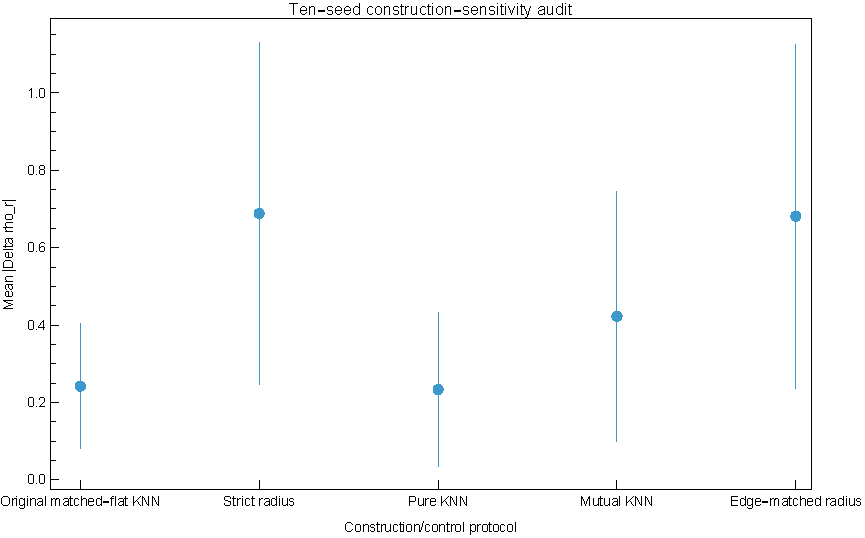
\includegraphics[width=0.78\linewidth]{results/figures/audit_mean_abs_gap.pdf}
    \caption{Mean absolute radial-correlation gap across the ten paired seeds.
    Error bars show sample standard deviation. The broad error bars are part of
    the result: protocol sensitivity and realization variability are both
    substantial.}
    \label{fig:audit-mean}
\end{figure}

The separation is not explained by a single edge-density comparison.
Table~\ref{tab:edge-counts} shows that strict radius and edge-matched radius give
nearly the same gap even though the former has a small seed-dependent edge-count
mismatch and the latter is exactly matched. Conversely, original and pure KNN
have similar mean absolute gaps despite very different black-hole edge rules.

\begin{table}[H]
\centering
\caption{Mean edge counts across ten seeds. The original protocol has a large
black-hole/flat density mismatch, whereas the other symmetric protocols are
approximately or exactly edge matched.}
\label{tab:edge-counts}
\small
\begin{tabular}{lrrr}
\toprule
Protocol & Mean BH edges & Mean flat edges & Mean BH--flat difference \\
\midrule
Original matched-flat KNN & 10171.2 & 9044.4 & 1126.8 \\
Strict radius             & 10171.2 & 10156.4 & 14.8 \\
Pure KNN                  & 9046.5  & 9044.4 & 2.1 \\
Mutual KNN                & 6953.5  & 6955.6 & -2.1 \\
Edge-matched radius       & 10171.2 & 10171.2 & 0.0 \\
\bottomrule
\end{tabular}
\end{table}

\subsection{Realization dependence and paired contrasts}

Figures~\ref{fig:audit-paired-abs} and~\ref{fig:audit-paired-signed} display the
same ten point samples across all protocols. The ordering is not identical from
seed to seed. Original, pure-KNN, and mutual-KNN gaps change sign in some
realizations; strict-radius and edge-matched-radius gaps are positive in all ten
runs. The original protocol contains one conventional $1.5\times\mathrm{IQR}$
outlier at seed 10, $\drho=0.6102$. Its graph, pairing, bins, connectivity, and
estimator-validity checks all pass, so it is retained.

\begin{figure}[H]
    \centering
    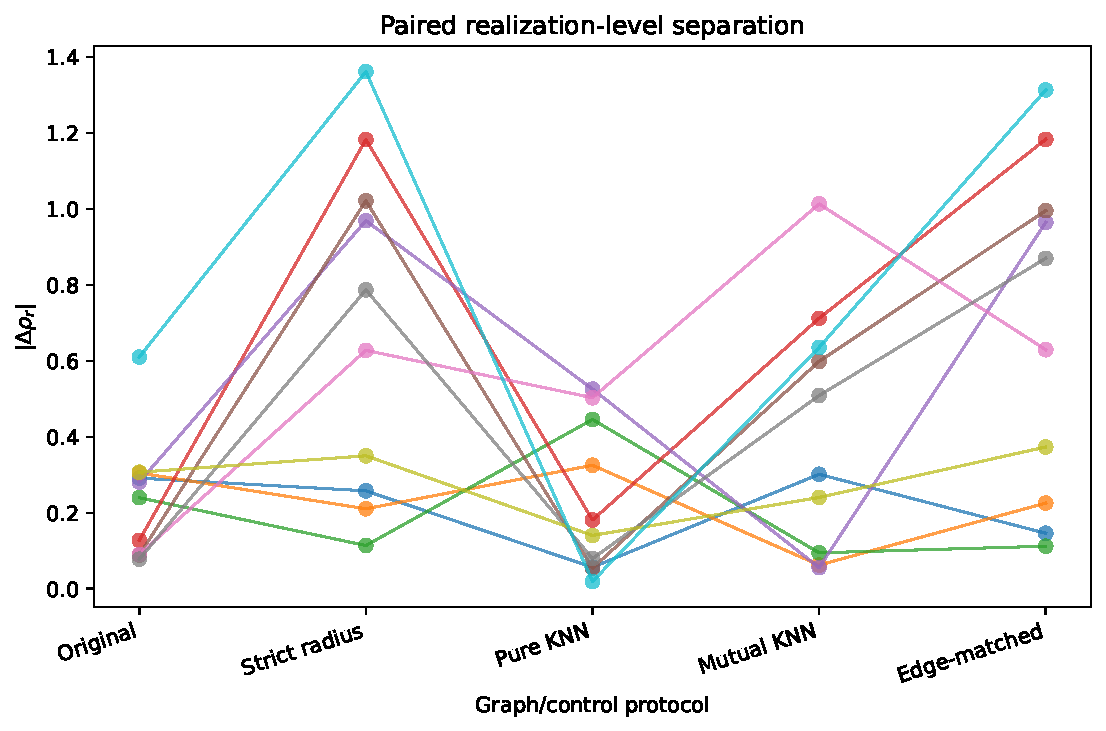
\includegraphics[width=0.90\linewidth]{results/figures/audit_paired_abs_gap.pdf}
    \caption{Paired $|\drho|$ values for all ten seeds. Lines join the same
    radial-angular sample across graph/control protocols.}
    \label{fig:audit-paired-abs}
\end{figure}

\begin{figure}[H]
    \centering
    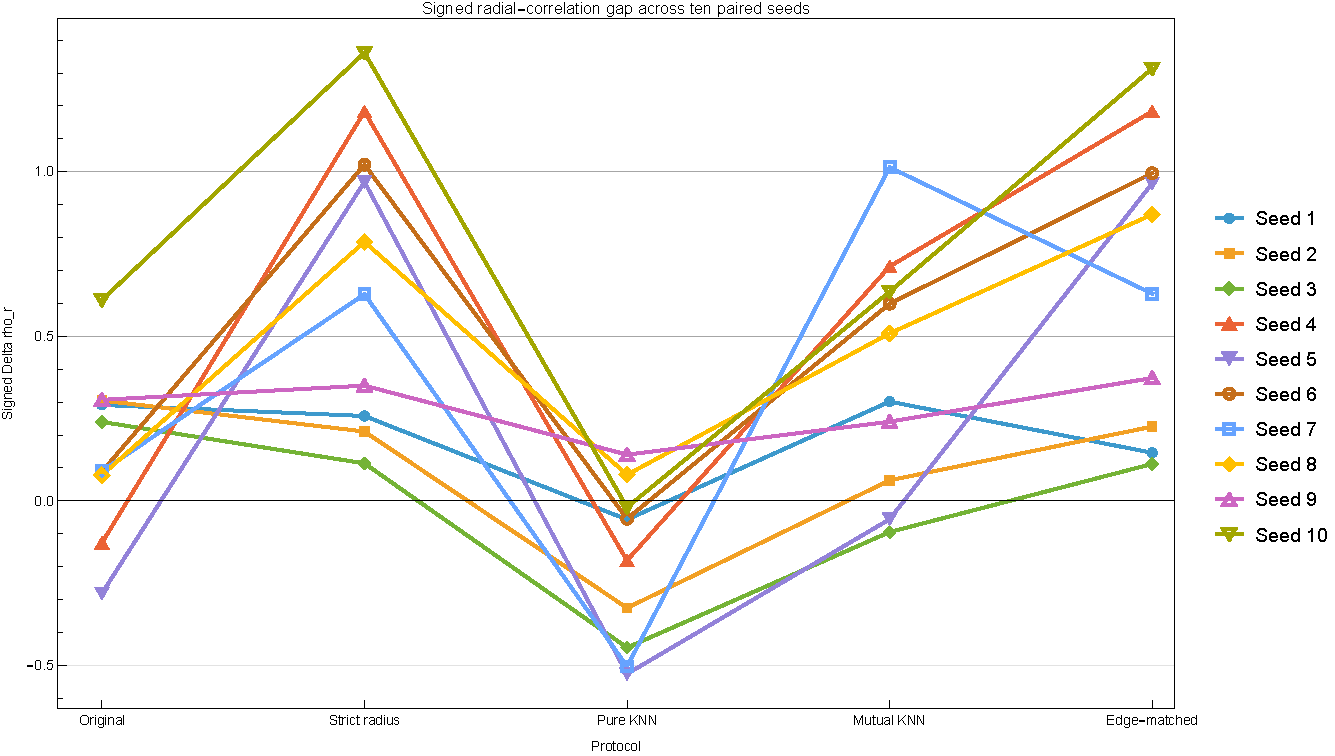
\includegraphics[width=0.90\linewidth]{results/figures/audit_paired_signed_gap.pdf}
    \caption{Signed $\drho$ for the same paired realizations. The sign changes
    show why signed and absolute gaps must be reported separately.}
    \label{fig:audit-paired-signed}
\end{figure}

Selected paired contrasts are given in Table~\ref{tab:paired-contrasts}. The
strict-radius and edge-matched-radius means exceed the original and pure-KNN
means in this sample, while strict radius and edge-matched radius are mutually
indistinguishable. These intervals quantify the paired experiment; they do not
establish a universal ranking of graph constructions.

\begin{table}[H]
\centering
\caption{Selected paired contrasts in $|\drho|$. The contrast is protocol A
minus protocol B; intervals are two-sided Student-$t$ intervals over ten paired
seeds.}
\label{tab:paired-contrasts}
\small
\resizebox{\linewidth}{!}{%
\begin{tabular}{llcc}
\toprule
Protocol A & Protocol B & Mean paired difference & 95\% CI \\
\midrule
Strict radius & Original matched-flat KNN & $0.446$ & $[0.122,0.771]$ \\
Strict radius & Pure KNN                  & $0.455$ & $[0.071,0.839]$ \\
Edge-matched radius & Original matched-flat KNN & $0.440$ & $[0.108,0.771]$ \\
Edge-matched radius & Pure KNN            & $0.448$ & $[0.066,0.831]$ \\
Strict radius & Edge-matched radius       & $0.007$ & $[-0.029,0.043]$ \\
Original matched-flat KNN & Pure KNN       & $0.009$ & $[-0.192,0.209]$ \\
\bottomrule
\end{tabular}%
}
\end{table}

\section{Canonical Bardeen and Hayward results}

The fixed-protocol scans quantify the family context that was previously only
illustrative. Table~\ref{tab:family-scans} reports mean $\pm$ sample standard
deviation over ten paired seeds. The flat-control values repeat across parameter
values because the same seed convention and radial-angular sampling law are
used. Increasing either regularization parameter changes the black-hole profile
gradually compared with the large realization spread. The black-hole common-bin
profile is negatively related to $\log K$ on average; for example, the mean
Pearson correlations at parameter $0.2$ are $-0.674\pm0.258$ (Bardeen) and
$-0.681\pm0.245$ (Hayward). These are associations on the same twelve bins, not
evidence that $\clog$ is a curvature scalar.

\begin{table}[H]
\centering
\caption{Canonical original-protocol family scans (mean $\pm$ SD, ten seeds).}
\label{tab:family-scans}
\small
\resizebox{\linewidth}{!}{%
\begin{tabular}{lcrrrr}
\toprule
Family & Parameter & $\rho_{\rm BH}$ & $\rho_{\rm flat}$ & $\drho$ & $|\drho|$ \\
\midrule
Bardeen & 0.0 & $0.592\pm0.266$ & $0.432\pm0.201$ & $0.160\pm0.250$ & $0.242\pm0.161$ \\
        & 0.1 & $0.587\pm0.275$ & $0.432\pm0.201$ & $0.155\pm0.258$ & $0.248\pm0.159$ \\
        & 0.2 & $0.581\pm0.293$ & $0.432\pm0.201$ & $0.149\pm0.279$ & $0.255\pm0.174$ \\
        & 0.3 & $0.563\pm0.331$ & $0.432\pm0.201$ & $0.131\pm0.316$ & $0.272\pm0.192$ \\
Hayward & 0.0 & $0.592\pm0.266$ & $0.432\pm0.201$ & $0.160\pm0.250$ & $0.242\pm0.161$ \\
        & 0.1 & $0.590\pm0.271$ & $0.432\pm0.201$ & $0.158\pm0.254$ & $0.246\pm0.159$ \\
        & 0.2 & $0.588\pm0.278$ & $0.432\pm0.201$ & $0.156\pm0.263$ & $0.250\pm0.165$ \\
        & 0.3 & $0.579\pm0.292$ & $0.432\pm0.201$ & $0.147\pm0.276$ & $0.254\pm0.169$ \\
\bottomrule
\end{tabular}%
}
\end{table}

\begin{figure}[H]
\centering
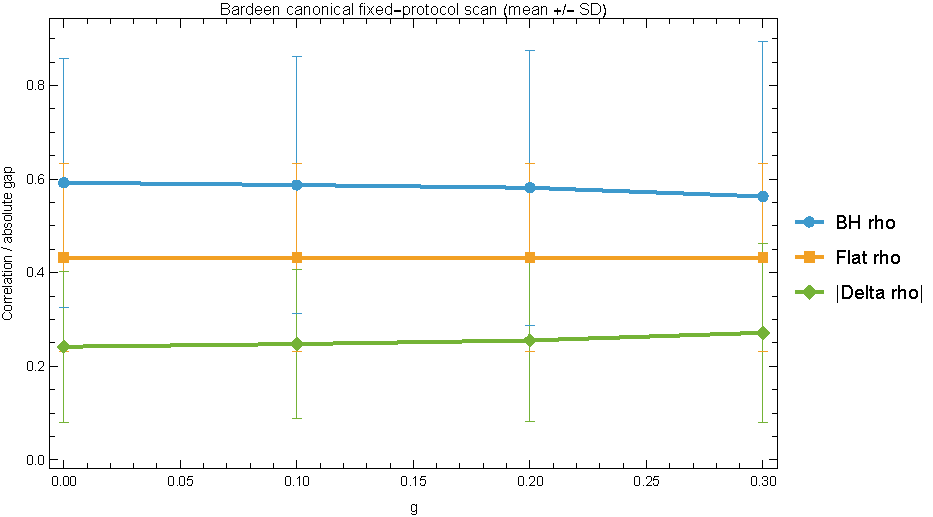
\includegraphics[width=.49\linewidth]{results/figures/bardeen_canonical_parameter_scan.pdf}
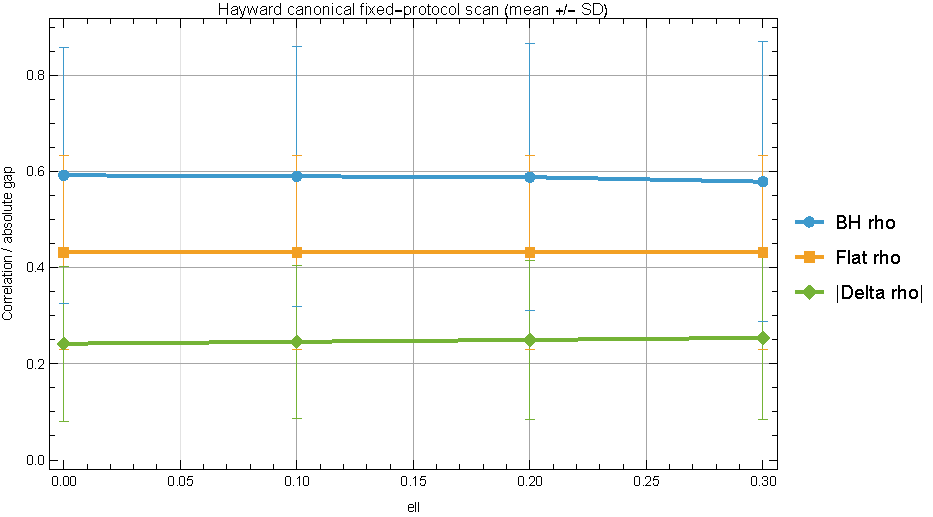
\includegraphics[width=.49\linewidth]{results/figures/hayward_canonical_parameter_scan.pdf}
\caption{Canonical Bardeen (left) and Hayward (right) parameter scans. Error
bars show sample SD across paired seeds.}
\label{fig:family-scans}
\end{figure}

The anchor audits show that the Schwarzschild construction sensitivity
generalizes qualitatively. For Bardeen, mean $|\drho|$ is $0.255\pm0.174$,
$0.678\pm0.435$, $0.211\pm0.170$, $0.422\pm0.322$, and $0.676\pm0.452$ in
protocol order. For Hayward the corresponding values are $0.250\pm0.165$,
$0.684\pm0.441$, $0.216\pm0.200$, $0.413\pm0.337$, and $0.680\pm0.443$.
Thus radius-style controls again give the largest average separation, but broad
paired variation precludes a universal protocol ranking.

\begin{figure}[H]
\centering
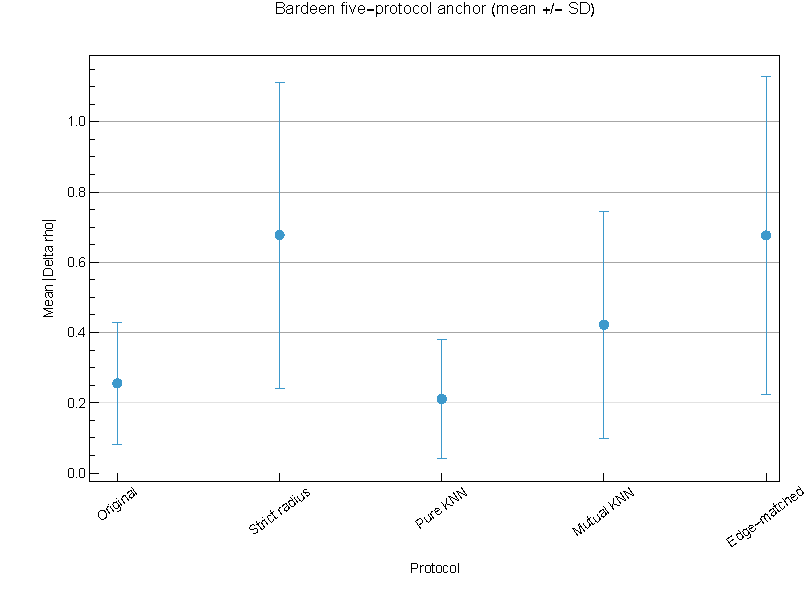
\includegraphics[width=.49\linewidth]{results/figures/bardeen_anchor_mean_abs_gap.pdf}
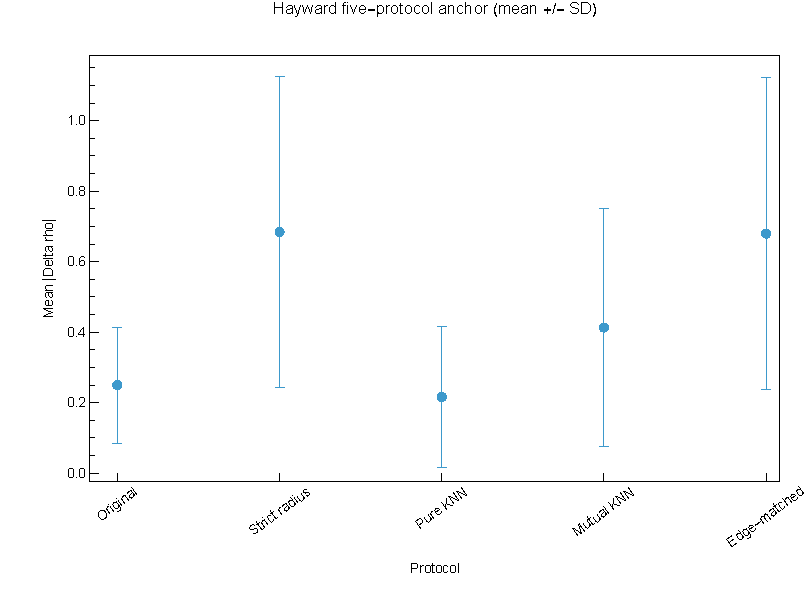
\includegraphics[width=.49\linewidth]{results/figures/hayward_anchor_mean_abs_gap.pdf}
\caption{Five-protocol anchors for Bardeen $g=0.2$ (left) and Hayward
$\ell=0.2$ (right), shown as mean $|\drho|\pm$ SD. Seed-level signed and
absolute plots are retained with the reproducibility outputs.}
\label{fig:family-anchors}
\end{figure}

The zero-parameter rows reproduce Schwarzschild row by row, not merely in
their means: coordinate hashes, common-profile hashes, and every exported
numeric output agree for each seed to tolerance $10^{-12}$ (maximum observed
difference zero). Unsupported legacy claims of a common $0.78$ gap and a
radius-control collapse to $10^{-3}$ are therefore removed rather than mixed
with the canonical pipeline.

\section{Discussion}

The paired audits change, but do not erase, the original result. $\clog$
displays organized radial behavior across the three black-hole embedding
families. The
question is whether the difference from a flat control is stable when the graph
representation changes. It is not. Both the magnitude and the sign of the gap
depend on the full protocol and on the random realization.

The most important correction is that radius-style controls do not absorb the
signal in any canonical anchor experiment. Strict-radius and edge-matched-radius
controls instead produce the largest mean absolute gaps. Their near equality is
especially informative: exact edge-count matching does not remove the effect,
and a small residual edge-count difference in the strict-radius protocol does
not explain it. At the same time, the broad seed-to-seed spread prevents a
universal protocol ranking.

The result supports a more precise interpretation of $\clog$. It is a statistic
of finite-shell shortest-path multiplicity organization. Shortest paths are
jointly determined by the sampled surface and by the imposed graph
representation. The appropriate object of interpretation is therefore
\begin{equation}
    \text{diagnostic} + \text{construction} + \text{control},
\end{equation}
not the diagnostic alone.

This distinction matters beyond black-hole embeddings. Geometric-graph studies
should report the sampling prescription, graph scale, edge rule, shell radius,
boundary handling, binning convention, seed distribution, and null-model
construction. At minimum, a geometric claim should be tested against a
sampling-matched control, a construction-matched control, and an edge-density
or edge-count-matched control.

\subsection{Scope and limitations}

The present experiment is a finite-graph benchmark, not a continuum curvature
reconstruction. It uses one graph size, one shell radius, one bin count, and ten
paired realizations. The confidence intervals are broad, and the analysis does
not establish continuum convergence. The graphs are built from Euclidean
embeddings of spatial slices; relationships to intrinsic two-dimensional
curvature, four-dimensional spacetime invariants, or non-embeddable data require
separate analysis.

The Bardeen and Hayward construction audits cover one representative parameter
each rather than the complete protocol-by-parameter matrix. The paper therefore
does not claim cross-family construction invariance or a universal ordering of
protocols. Multi-resolution runs, shell-radius sweeps, alternative binning,
additional parameter anchors, and canonical audits of other diagnostics remain
useful extensions.

\subsection{Reproducibility}

The new calculation contains exactly 80 family-scan rows and 100 anchor-audit
rows, with no missing family, parameter, seed, or protocol. All primary and
secondary correlations are numeric, every run contains twelve common radial
bins, and the maximum radial-angular mismatch is $1.33\times10^{-15}$. Complete
vertex sets, connectivity, valid-$\clog$ fractions, mutual-KNN subset checks,
and exact or tie-explained edge matching are recorded. The 100 checkpoint units
required $27701.3$ seconds ($7.69$ h) of compute time, ranging from $116.5$ to
$1099.9$ seconds per checkpoint. The preceding Schwarzschild audit required
$3636.84$ seconds.

Code, scripts, raw data, quality-control tables, checkpoints, validation files,
and manuscript figures are available in the \href{https://github.com/Uxuee/PathAnisotropyCurvature}{project repository}. A DOI-backed archival snapshot should accompany journal submission.

\section{Conclusion}

We studied the shortest-path anisotropy statistic $\clog$ on geometric graphs
sampled from embedded black-hole spatial slices. Canonical ten-seed Bardeen and
Hayward scans show organized radial behavior under one fixed protocol, with
family-parameter and realization dependence. Paired five-protocol audits at
Schwarzschild and representative Bardeen and Hayward anchors test how the
black-hole/control separation changes with graph construction.

The audit does not confirm the earlier claim that radius-style controls erase
the gap. Strict-radius and edge-matched-radius constructions instead produce the
largest mean absolute separations, whereas the original and pure-KNN protocols
produce smaller averages. Signed gaps vary across realizations and reverse under
some protocols. The separation is therefore neither graph-construction
invariant nor realization independent.

The main conclusion is methodological. $\clog$ is a reproducible finite-shell
shortest-path statistic under fully specified conditions, but it is not a
graph-independent curvature scalar. Apparent geometric signals in spatial graph
diagnostics should be interpreted as properties of complete
 diagnostic--construction--control protocols. The anchor results show that
strong construction dependence is shared across the three tested families,
while limited parameter, resolution, and shell coverage prevents a
graph-independent curvature interpretation.

\section*{Funding}

This research received no specific grant from any funding agency in the
public, commercial, or not-for-profit sectors.

\section*{Data and code availability}

A versioned archive of the code and data will be deposited in Zenodo upon
release. The DOI will be inserted before journal submission.

\begin{thebibliography}{99}

\bibitem{Penrose2003}
M. Penrose,
\emph{Random Geometric Graphs}.
Oxford University Press, Oxford, 2003.

\bibitem{DallChristensen2002}
J. Dall and M. Christensen,
Random geometric graphs,
\emph{Physical Review E} \textbf{66}, 016121 (2002).

\bibitem{Newman2010}
M. E. J. Newman,
\emph{Networks: An Introduction}.
Oxford University Press, Oxford, 2010.

\bibitem{VanWijk2010}
B. C. M. van Wijk, C. J. Stam, and A. Daffertshofer,
Comparing brain networks of different size and connectivity density using graph
theory,
\emph{PLoS ONE} \textbf{5}, e13701 (2010).

\bibitem{Langer2013}
N. Langer, A. Pedroni, and L. J{\"a}ncke,
The problem of thresholding in small-world network analysis,
\emph{PLoS ONE} \textbf{8}, e53199 (2013).

\bibitem{Ginestet2011}
C. E. Ginestet, T. E. Nichols, E. T. Bullmore, and A. Simmons,
Brain network analysis: separating cost from topology using cost-integration,
\emph{PLoS ONE} \textbf{6}, e21570 (2011).

\bibitem{Regge1961}
T. Regge,
General relativity without coordinates,
\emph{Nuovo Cimento} \textbf{19}, 558--571 (1961).

\bibitem{Forman2003}
R. Forman,
Bochner's method for cell complexes and combinatorial Ricci curvature,
\emph{Discrete \& Computational Geometry} \textbf{29}, 323--374 (2003).

\bibitem{Ollivier2009}
Y. Ollivier,
Ricci curvature of Markov chains on metric spaces,
\emph{Journal of Functional Analysis} \textbf{256}, 810--864 (2009).

\bibitem{Schwarzschild1916}
K. Schwarzschild,
{\"U}ber das Gravitationsfeld eines Massenpunktes nach der Einsteinschen Theorie,
\emph{Sitzungsberichte der K{\"o}niglich Preussischen Akademie der Wissenschaften}
189--196 (1916).

\bibitem{Flamm1916}
L. Flamm,
Beitr{\"a}ge zur Einsteinschen Gravitationstheorie,
\emph{Physikalische Zeitschrift} \textbf{17}, 448--454 (1916).

\bibitem{Bardeen1968}
J. M. Bardeen,
Non-singular general-relativistic gravitational collapse,
in \emph{Proceedings of the International Conference GR5}, Tbilisi, USSR, p. 174
(1968).

\bibitem{Hayward2006}
S. A. Hayward,
Formation and evaporation of nonsingular black holes,
\emph{Physical Review Letters} \textbf{96}, 031103 (2006).

\end{thebibliography}

\end{document}
